\section{Introduction}

Bubbles within liquids are incredibly common, occurring in both a wide spectrum of natural and industrial processes \cite{veron2015ocean}. These occurrences can range from water and carbon-dioxide bubbles in magma providing driving forces for an eruption \cite{Volcano} to carbon-dioxide bubbles in champagne enhancing the evaporation of volatile organic compounds dispersed in the liquid phase \cite{WINE}. When a bubble rises to the surface of a liquid, it may burst, scattering many droplets. These droplets are an important process of transport exchange across the liquid gas interface, they are considered the main source of sea spray aerosols \cite{veron2015ocean} and impact air pollution \cite{murphy2016depth} as well as the transmission of infectious diseases \cite{ji2022water,bourouiba2021fluid}. Bubbles formed due to the breaking of waves contribute to the transfer of heat, mass and other contaminants between the oceans and the atmosphere \cite{coantic1980mass}. The formation of ocean spray by bursting bubbles in coastal areas during red tides of harmful algae can bring pathogens into the atmosphere as aerosols causing heath issues \cite{walls2014moving}. The efficiency of this transfer is governed by the initial size and speed of the ejected drops. \cite{coantic1980mass,andreas1995spray}

\begin{figure}[H]
    \centering
    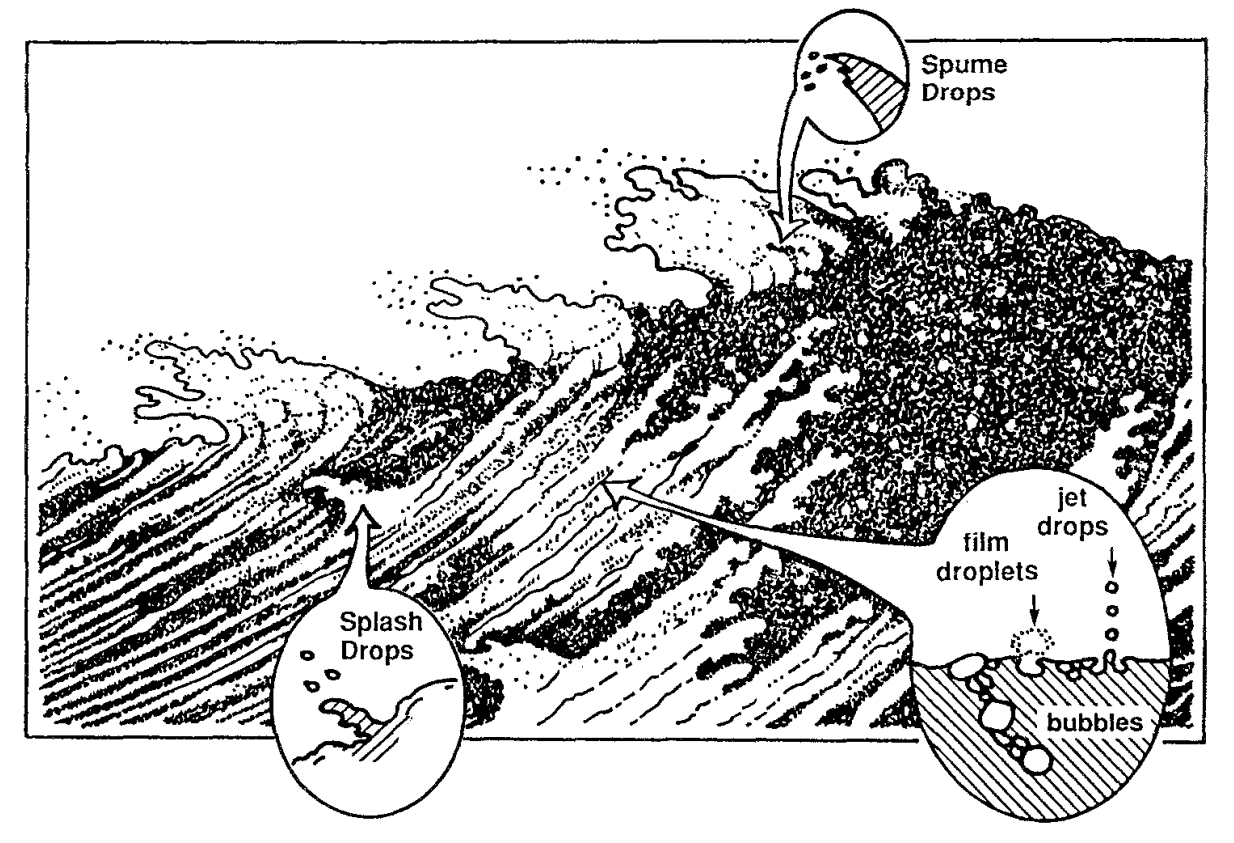
\includegraphics[width=0.8\linewidth]{WriteUp/images/Andreas pic.png}
    \caption{Origin of the various kinds of sea spray droplet. This report focuses on Jet drops Adapted from figure 1 on page 5 of Andreas \textit{et al.} \cite{andreas1995spray} }
    \label{fig:0}
\end{figure}

There are two phenomena that occur when a bubble bursts that produce aerosols, the first being when the thin film separating the bubble from the atmosphere is ruptured. The atomisation of the film can produce several hundred droplets of around a micrometer in diameter. Due to the length scales of the rupture being order O($100$)nm \cite{boulton1993gas}, we are unable to describe this problem with continuum mechanics. In fact, van der Waals forces or electrostatic repulsion must be considered, both of which are long-range intermolecular forces \cite{boulton1993gas}. 

After the film rupture, the remaining cavity collapses causing a jet to form. This jet eventually breaches into one or more droplets. The key difference between these droplets and the droplets formed when the film ruptures is that they are much larger, order O($100 \mu$m) for a typical bubble with a diameter of a millimeter. They are also ejected vertically with a typical ejection velecity of order O($1$ms$^{-1}$).
\begin{figure}[H]
    \centering
    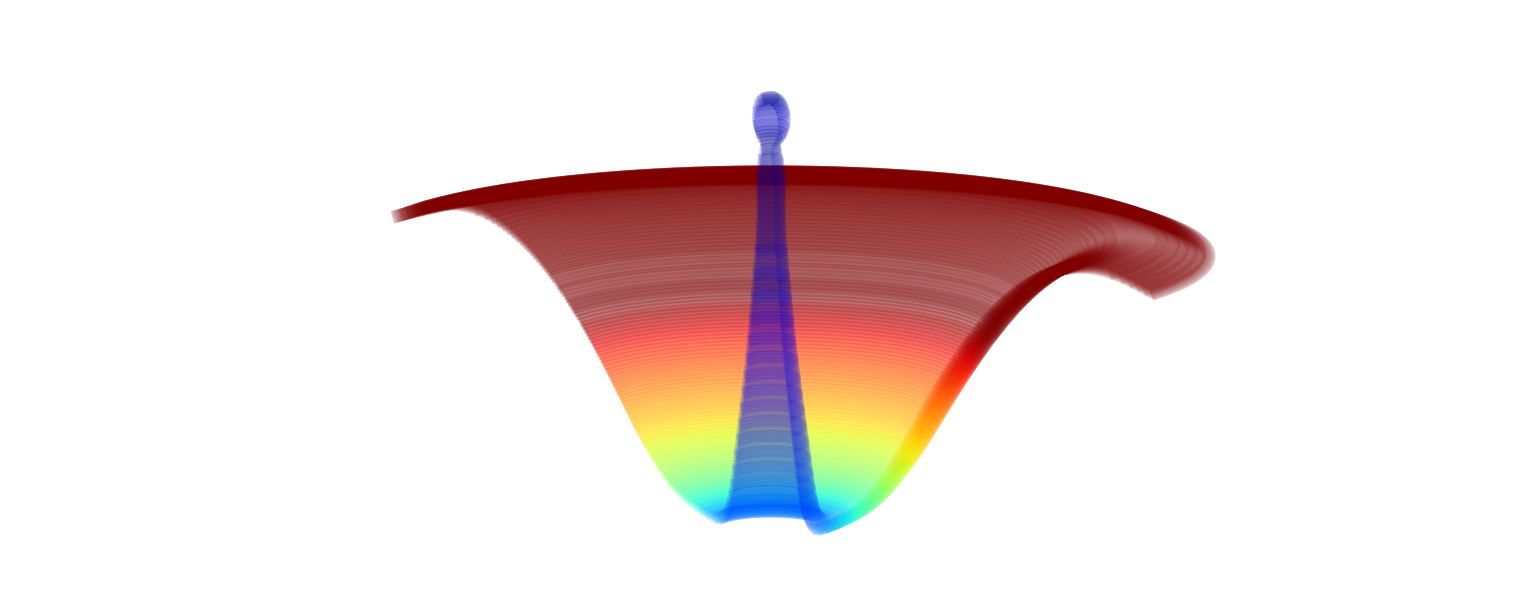
\includegraphics[width=0.75\linewidth]{WriteUp/images/droplet release 3D.png}
    \caption{An image of jet formation due to a burst bubble.}
    \label{fig:1}
\end{figure}

Since the pioneering study of bursting bubbles by Woodcock \textit{et al.} \cite{woodcock1953giant}, numerous studies have been made documenting jet drop properties. The first comprehensive study using numerical simulations based on a free-surface formulation of the Navier-Stokes equations was done in 2002 by Duchemin \textit{et al.} \cite{duchemin2002jet
}.

In this paper they used a volume-of-fluid (VOF) type method to investigate quantities such as the jet velocity, maximum pressure on the axis of symmetry and radius of the first ejected drop. They compared their numerical data with experimental data published by MacIntyre \cite{macintyre1972flow} and found the overall agreement satisfactory. The method was able to resolve small capillary wave and still accurately predict large scale features of the dynamics, the pressure and final droplet radius.

Another aim of this paper was to investigate bubble entrapment. This is when a new bubble is formed underneath the collapsing cavity of the old bubble. Two entrapment regions were found, the first for $576<R/R_v<2016$ and the second between $57\:600<R/R_v<288\:000$ where $R$ is the radius of the bubble and $R_v=\rho\nu^2/\gamma$ is the viscous-capillary length with $\rho$, $\nu$ and $\gamma$ being liquid density, kinematic viscosity and surface tension respectively. Other regions of entrapment at higher values of $R/R_v$ was speculated but was said to be difficult to observe numerically.

Duchemin \textit{et al.} also showed that the jets are produced by the self-similar collapse of a cavity created by capillary waves. When a bubble cavity is collapsing, small waves form on the cavity interface moving towards the centre of the bubble. due to the symmetrical nature of the phenomenon these waves focus at the centre of the bubble causing a jet to form. These dynamics can be described by a self-similar dynamic based on the balance of inertial and capillary forces \cite{brenner2000jets} and leads to a singularity where the velocity diverges although in reality it is regularised by viscous and capillary effects. Viscosity was shown to play a critical role in the formation of this singularity. Counter-intuitively, the fastest jets are not obtained for a vanishing viscosity, rather they occur in a small range of optimal viscosity. For a Laplace number $\text{La}=\gamma R\rho/\mu^2$ of around $1000$ where $\mu$ is dynamic viscosity, approaches a finite-time singularity for both pressure and velocity. \cite{brenner2000jets} Earlier attempts of numerical simulation used boundary integral methods for inviscid fluids and therefore missed this phenomenon \cite{oguz1993dynamics}.

However, the paper by Duchemin \textit{et al.} was not entirely comprehensive. Many aspects of busting bubbles were not considers, in particular gravity. This lead to a simplified initial condition of a spherical bubble lying just beneath the surface. A hole was then put into the bubble and the sharp edges left over were smoothed to try and prevent numerical singularities. In addition, due to the limited availability fo experimental data at the time, comparisons between the numerical simulations and experimental data was limited and qualitative.

Deike \textit{et al.} tried to rectify these shortcomings in an article where they aimed to verify experimental and numerical results were indeed quantitatively consistent and obtain a complete quantitative description of how the jet velocity depends on both viscosity and gravity and attempt to separate these two effects \cite{deike2018dynamics}. The authors showed that due to the transient nature of the jet formation process, trying to define the jet velocity is incredibly difficult. as a result, throughout the literature there were numerous definitions leading to conflicting reported velocities. They defined the jet velocity as the stationary velocity observed before drop ejection which they found was consistent with most of the experimental measurements \cite{spiel1995births}. They discussed scaling laws involving the Weber number $\text{We}=\rho v^2R/\gamma$ where $v$ is the velocity of the jet, the capillary number $\text{Ca}=\mu v/\gamma$, the Laplace number and the Bond number. They found $\text{We} \propto \text{Bo}^{\beta}$ and $\text{Ca} \propto \text{Bo}^{\beta}$ where $\beta$ depends on the Bond and Laplace numbers. As gravity was now being considered, a more complicated initial condition was used and through direct numerical simulation they were able to separate the roll of gravity (through the Bond number) and viscosity (through the Laplace number). A universal formula was presented linking the jet capillary number to the Bond and Laplace number and found optimal Laplace numbers depending on the Bond number and that the highest velocity is reached for vanishing Bond numbers. When calculating results with $\text{Bo}=0$ they acquired results compatible with what Duchemin \textit{et al.} had done.

Work has also been done into bursting bubble problems involving a third phase like oil. Yang \textit{et al.} \cite{yang2023enhanced} looked into the case where oil coated the inside of the bubble. They found the air-oil-water interface offered a distinct meachanism to smooth initial capillary waves during cavity collapse. This leads to a more efficient focusing of the larger waves, allowing singular jets to form over a larger parameter space and jet droplets to form on a much smaller scale.

In this report we investigate the effect of the initial condition on parameters such as jet velocity and time of ejection. Calculating the initial condition is difficult and time consuming, if we able able to determin a region in which it is sufficient to use a simplified initial condition we would be able to accelerate further research by reducing simulation time.

The report is structured as follows. In section 2 we give an overview of the scaling laws present in the problem and how we are able to derive them. In section 3 we calculate the initial shape of the bubble before bursting. This is done by first deriving the equations governing the system, transforming them into equations that are able to be solved numerically and finally by implementing a numerical solution in Python. In section 4 we give details on the how we compute the bubble interface evolving in time and compare results obtained by using the initial conditions we calculate in section 3 and the simplified initial conditions as used by Duchemin \textit{et al.} \cite{duchemin2002jet}. In section 5 we conclude with a summary of the effectiveness of the simplified initial condition and in which directions the problem of bursting bubble could be taken.